\chapter{Schedule}

This project requires a meticulously planned roadmap to navigate the complexities and milestones that lie ahead. The Gantt Chart in Figure \ref{fig:project-gantt-chart} serves as a visual compass, delineating the chronological sequence of tasks and deadlines essential for the successful completion of the project. Each bar, carefully plotted along the timeline, represents a crucial aspect of the thesis development process, offering a comprehensive overview of the project's progression. This dynamic tool not only aids in project management but also provides a clear visualization of interdependencies, helping to anticipate potential challenges and facilitating effective decision-making throughout the thesis endeavor.

\begin{figure} [H]
    \centering
    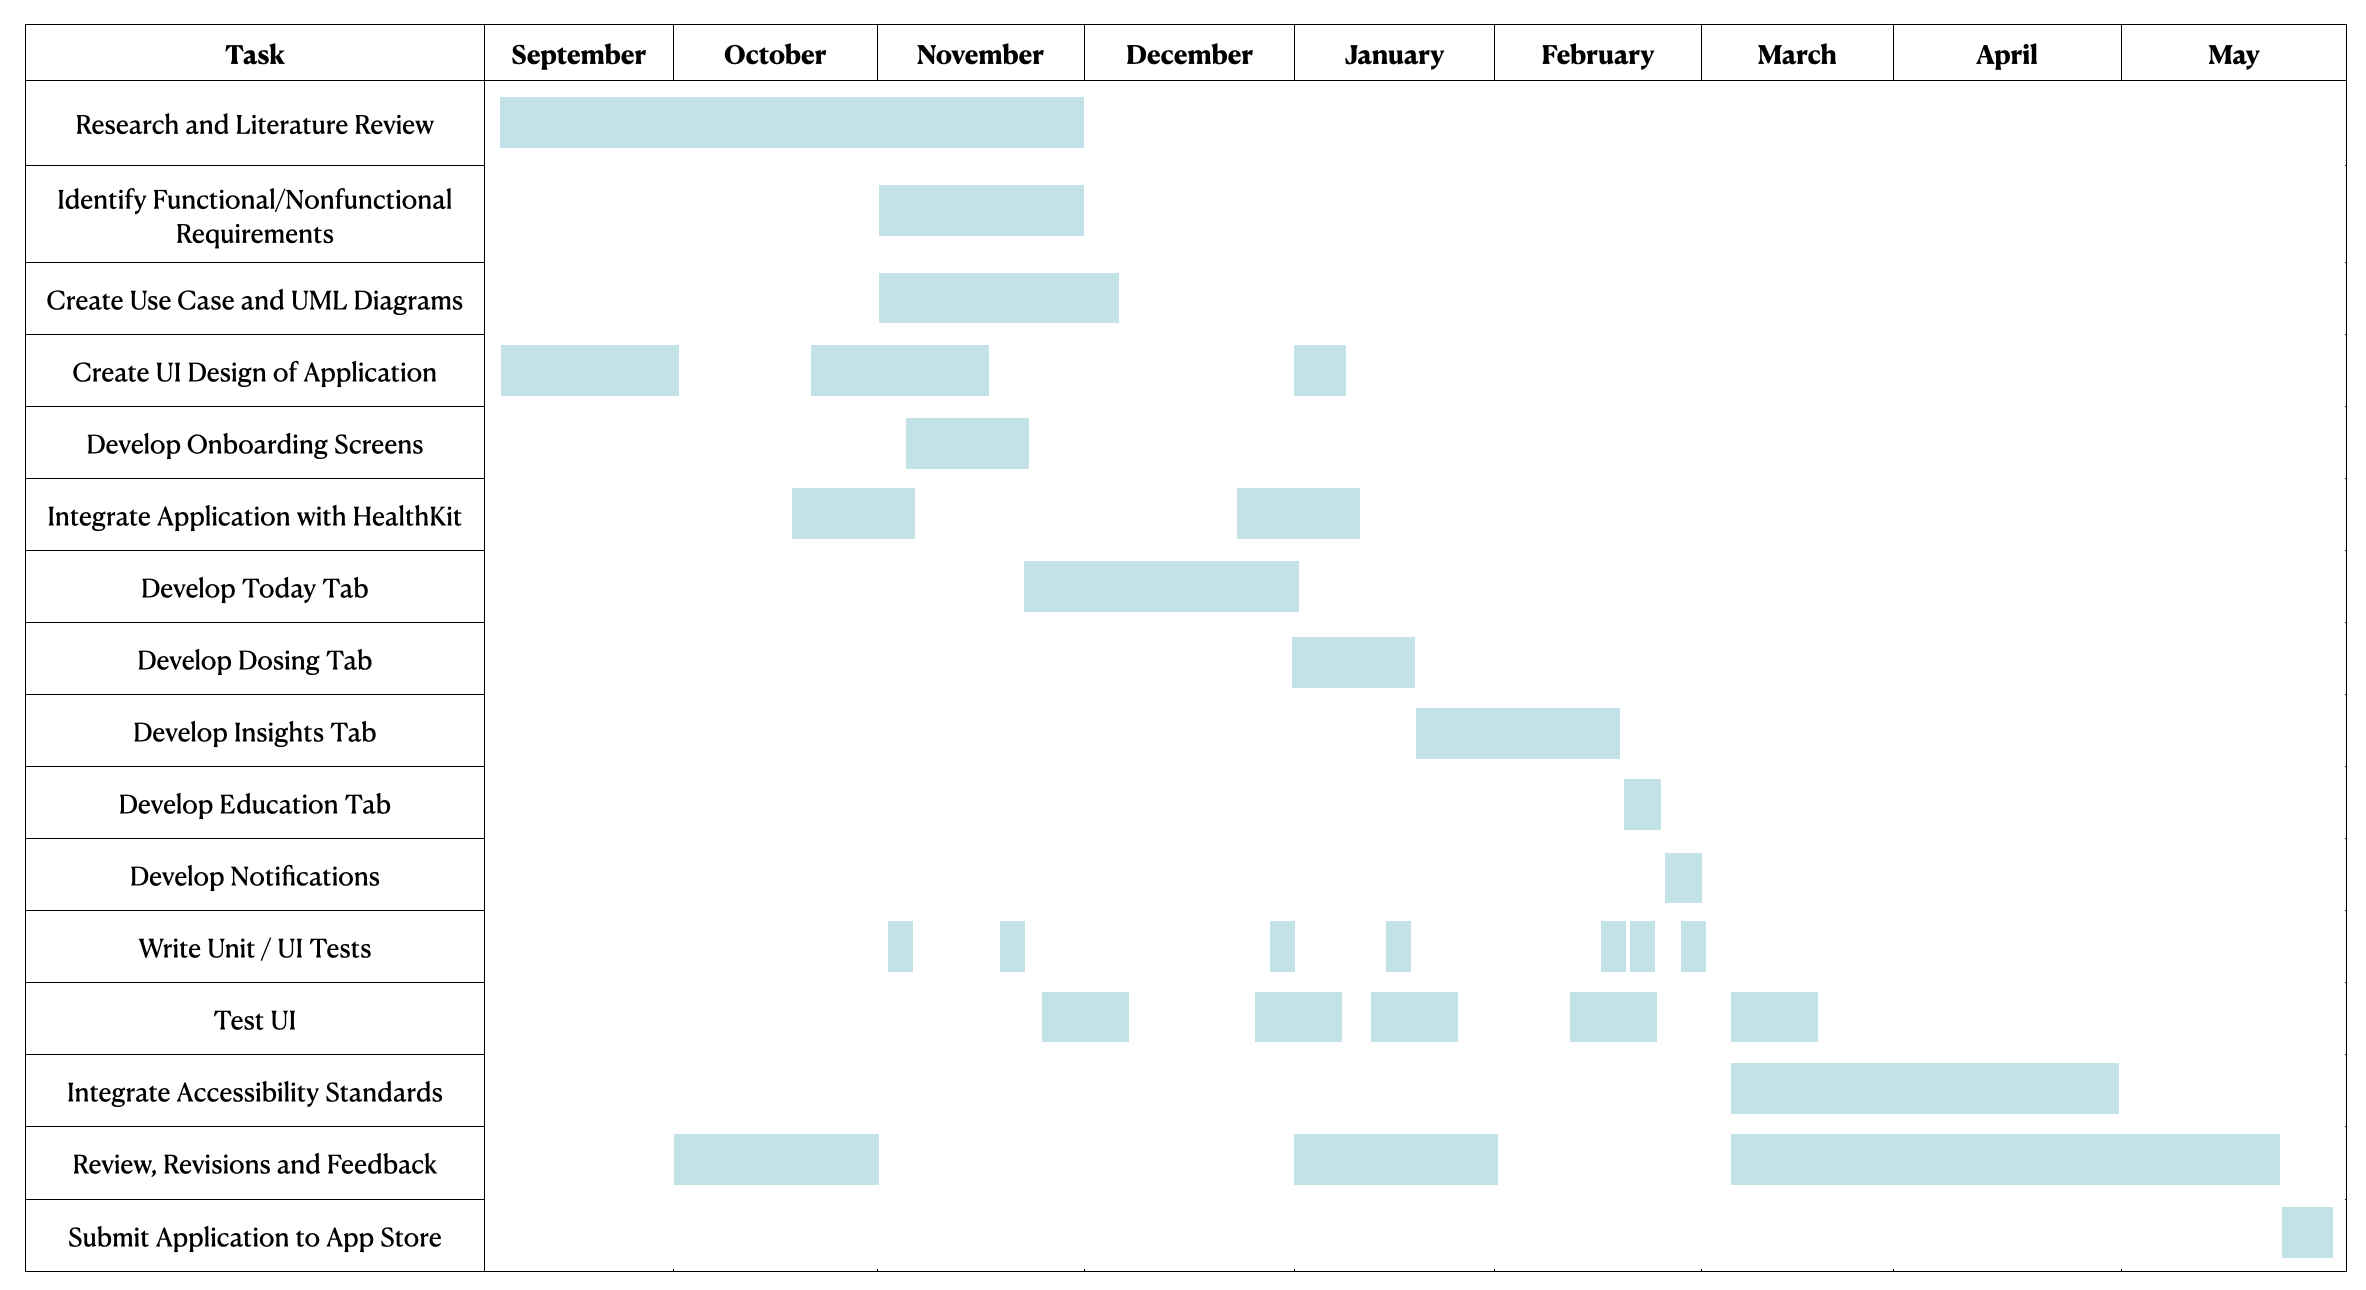
\includegraphics[width=1\linewidth]{thesis//chapters//images/ganttChart.png}
    \caption{Project Gantt Chart}
    \label{fig:project-gantt-chart}
\end{figure}

